\graphicspath{{./sixth/img}}

\section*{\LARGE{Введение}}
\addcontentsline{toc}{section}{Введение}
\textbf{Цель}: научиться работать с ресурсами в Android Studio.\par
Ресурс в приложении Android представляет собой файл, например, файл
разметки интерфейса или некоторое значение, например, простую строку. То
есть ресурсы представляют собой и файлы разметки, и отдельные строки, и
звуковые файлы, файлы изображений и т.д. Все ресурсы находятся в проекте
в каталоге res. Для различных типов ресурсов, определенных в проекте, в
каталоге res создаются подкаталоги. Поддерживаемые подкаталоги:

\begin{itemize}
	\item animator/: xml-файлы, определяющие анимацию свойств;
	\item anim/: xml-файлы, определяющие tween-анимацию;
	\item color/: xml-файлы, определяющие список цветов;
	\item drawable/: Графические файлы (.png, .jpg, .gif);
	\item mipmap/: Графические файлы, используемые для иконок приложения;
		под различные разрешения экранов;
	\item layout/: xml-файлы, определяющие пользовательский интерфейс
		приложения;
	\item menu/: xml-файлы, определяющие меню приложения;
	\item raw/: различные файлы, которые сохраняются в исходном виде;
	\item values/: xml-файлы, которые содержат различные используемые в
		приложении значения, например, ресурсы строк;
	\item xml/: Произвольные xml-файлы;
	\item font/: файлы с определениями шрифтом и расширениями .ttf, .otf или
		.ttc, либо файлы XML, который содержат элемент <font-family>.
\end{itemize}

Существует два способа доступа к ресурсам: в файле исходного кода и в
файле xml.
Ссылка на ресурсы в коде
Тип ресурса в данной записи ссылается на одно из пространств (вложенных
классов), определенных в файле R.java, которые имеют соответствующие им
типы в xml:

\begin{itemize}
	\item R.drawable (ему соответствует тип в xml drawable);
	\item R.id (id);
	\item R.layout (layout);
	\item R.string (string);
	\item R.attr (attr);
	\item R.plural (plurals);
	\item R.array (string-array).
\end{itemize}

Нередко возникает необходимость ссылаться на ресурс в файле xml,
например, в файле, который определяет визуальный интерфейс, к примеру, в
activity\_main.xml. Ссылки на ресурсы в файлах xml имеют следующую
формализованную форму: \verb|@[имя_пакета:]тип_ресурса/имя_ресурса|. Где:
\begin{itemize}
	\item имя\_пакета представляет имя пакета, в котором ресурс находится
		(указывать необязательно, если ресурс находится в том же пакете);
	\item тип\_ресурса представляет подкласс, определенный в классе R для
		типа ресурса;
	\item имя\_ресурса имя файла ресурса без расширения или значение
		атрибута android:name в XML-элементе (для простых значений).
\end{itemize}

\clearpage

\section*{\LARGE{Выполнение практической работы}}
\addcontentsline{toc}{section}{Выполнение практической работы}

\section{Ресурсы строк}
Ресурсы строк --- один из важных компонентов приложения. Мы используем
их при выведении названия приложения, различного текста, например, текста
кнопок и т.д.\par
XML-файлы, представляющие собой ресурсы строк, находятся в проекте в
каталоге res/values. По умолчанию ресурсы строк находятся в файле strings.xml,
который может выглядеть следующим образом.\par
Пример использования ресурса проиллюстрирован на
рисунках~\ref{fig:xml:string}\,-\,\ref{fig:java:string}.

\begin{image}
	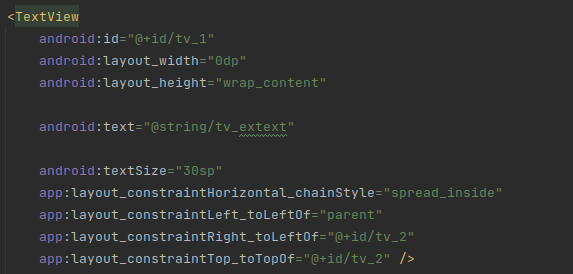
\includegraphics[width=0.9\textwidth]{Screenshot from 2023-03-28 15-20-22}
	\caption{Использование ресурсов строк в XML-коде}
	\label{fig:xml:string}
\end{image}

\begin{image}
	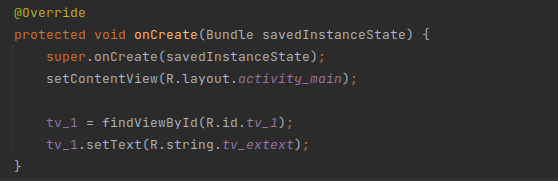
\includegraphics[width=0.9\textwidth]{Screenshot from 2023-03-28 15-30-24}
	\caption{Использование ресурсов строк в Java-коде}
	\label{fig:java:string}
\end{image}

\section{Форматирование строк}
Android позволяет применять к ресурсам строк форматирование. Пример
показан на рисунке~\ref{fig:format:string}.

\begin{image}
	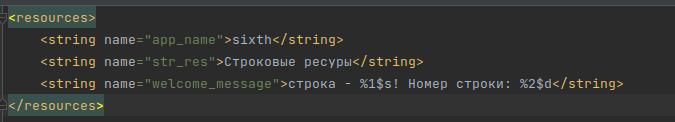
\includegraphics[width=0.9\textwidth]{Screenshot from 2023-03-28 15-40-34}
	\caption{Форматная строка в каталоге ресурсов}
	\label{fig:format:string}
\end{image}

Пример использования форматированной строки проиллюстрирован
на рисунках~\ref{fig:java:format}.

\begin{image}
	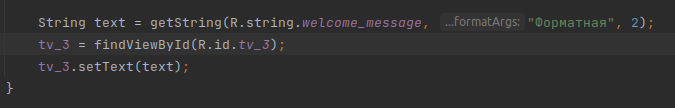
\includegraphics[width=0.9\textwidth]{Screenshot from 2023-03-28 15-44-46}
	\caption{Использование форматной строки в Java-коде}
	\label{fig:java:format}
\end{image}

\section{Ресурсы Plurals}
Plurals представляют еще один вид набора строк.
Ресурс plurals используется, напрмер если нужно использовать одно
существительное с разными окончаниями, изменяемое в зависимости от
числительного, которое с ним употребляется: 1 колотушка, 2 колотушки,
5 колотушек.\par
Пример файла ресурсов изображен на рисунке~\ref{fig:xml:plurals}.

\begin{image}
	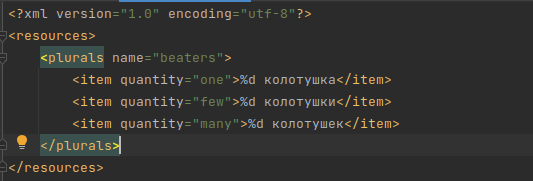
\includegraphics[width=0.9\textwidth]{Screenshot from 2023-03-30 18-44-25}
	\caption{Объявление ресурсов Plurals}
	\label{fig:xml:plurals}
\end{image}

Для задания ресурса используется элемент \texttt{<plurals>}, для которого
существует атрибут \texttt{name}, получающий в качестве значения произвольное
название, по которому потом ссылаются на данный ресурс.\par
Сами наборы строк вводятся дочерними элементами \texttt{<item>}. Этот элемент
имеет атрибут \texttt{quantity}, который имеет значение, указывающее,
когда эта строка используется. Данный атрибут может принимать следующие
значения:

\begin{itemize}
	\item zero: строка для количества в размере 0;
	\item one: строка для количества в размере 1 (для русского языка - для
		задания всех количеств, оканчивающихся на 1, кроме 11);
	\item two: строка для количества в размере 2;
	\item few: строка для небольшого количества.
\end{itemize}

Причем в данном случае многое зависит от конкретного языка. А система
сама позволяет определить, какое значение брать для того или иного числа.

С помощью метода \texttt{getQuantityString} можно получить значение ресурса.
Первым параметром передаем идентификатор ресурса. Вторым параметром
идет значение. для которого нужно найти нужную строку. Третий параметр
представляет собой значение, которое будет вставляться на место
плейсхолдера \%d. То есть получается строка для числа 21.\par
Пример показан на рисунке~\ref{fig:java:plurals}.

\begin{image}
	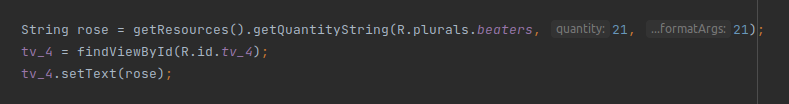
\includegraphics[width=0.9\textwidth]{Screenshot from 2023-03-30 19-03-46}
	\caption{Использование ресурсов Plurals в Java-коде}
	\label{fig:java:plurals}
\end{image}

\section{String array}
Еще одним видом строковых ресурсов является string-array или массив строк.
Ресурс задается с помощью элемента \texttt{<string-array>}. Фактически он
определяет набор строк. А каждая отдельная строка задается с помощью
элемента \texttt{<item>}.
Пример кода показан на рисунке~\ref{fig:xml:array}.

\begin{image}
	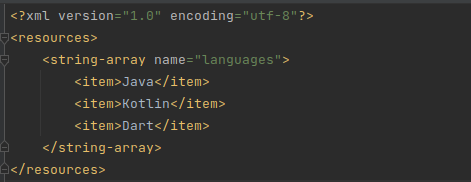
\includegraphics[width=0.9\textwidth]{Screenshot from 2023-03-30 19-09-10}
	\caption{Объявление ресурсов string array}
	\label{fig:xml:array}
\end{image}

С помощью метода getStringArray получаем ресурс в массив строк и затем с
помощью цикла сложили из массива одну строку и передаем ее в TextView.
(Рисунок~\ref{fig:java:array}).

\begin{image}
	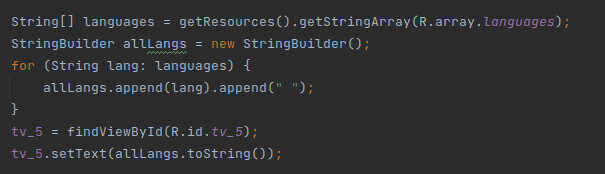
\includegraphics[width=0.9\textwidth]{Screenshot from 2023-03-30 19-13-31}
	\caption{Использование ресурсов string array в Java-коде}
	\label{fig:java:array}
\end{image}

\section{Ресурсы dimension}
Определение размеров должно находиться в каталоге res/values в файле с
любым произвольным именем. Общий синтаксис определения ресурса показан,
на рисунке~\ref{fig:xml:dimension}.

\begin{image}
	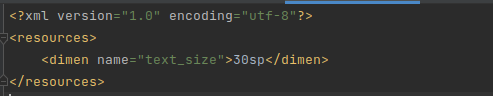
\includegraphics[width=0.9\textwidth]{Screenshot from 2023-03-30 19-18-23}
	\caption{Объявление ресурсов dimension}
	\label{fig:xml:dimension}
\end{image}

Как и другие ресурсы, ресурс dimension определяется в корневом элементе
\texttt{<resources>}. Тег \texttt{<dimen>} обозначает ресурс и в качестве
значния принимает некоторое значение размера в одной из принятых единиц
измерения (dp, sp, pt, px, mm, in). Более подробно установка размеров
рассматривалась в одной из прошлых практических занятий.\par
Пример использования ресурса показан на
рисунках~\ref{fig:xml:dimension:use}\,-\,\ref{fig:java:dimension:use}.

\begin{image}
	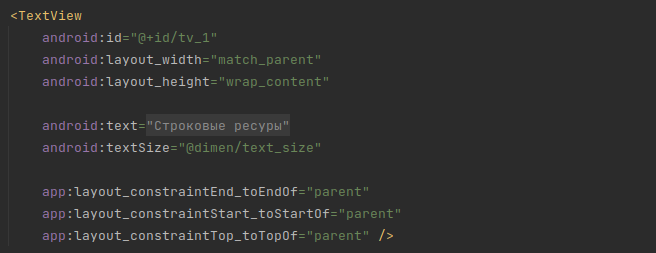
\includegraphics[width=0.9\textwidth]{Screenshot from 2023-03-30 19-21-28}
	\caption{Использование ресурсов dimension в XML-коде}
	\label{fig:xml:dimension:use}
\end{image}

\begin{image}
	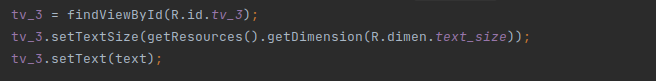
\includegraphics[width=0.9\textwidth]{Screenshot from 2023-03-30 19-44-25}
	\caption{Использование ресурсов dimension в Java-коде}
	\label{fig:java:dimension:use}
\end{image}

Для получения ресурсов в коде java применяется метод \texttt{getDimension()}
класса \texttt{Resources}.

\section{Ресурсы Color}
В приложении Android также можно определять ресурсы цветов (Color). Они
должны храниться в файле по пути res/values и также, как и ресурсы строк,
заключены в тег \texttt{<resources>}. Так, по умолчанию при создании самого
простого проекта в папку res/values добавляется файл colors.xml
(Рисунок~\ref{fig:xml:color}).

\begin{image}
	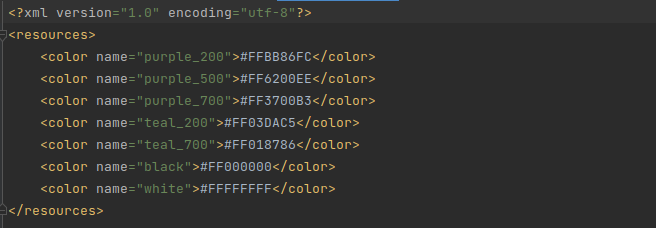
\includegraphics[width=0.9\textwidth]{Screenshot from 2023-03-30 19-25-31}
	\caption{Объявление ресурсов colors}
	\label{fig:xml:color}
\end{image}

Цвет определяется с помощью элемента \texttt{<color>}. Его атрибут
\texttt{name} устанавливает название цвета, которое будет использоваться
в приложении, а шестнадцатеричное число --- значение цвета.
Для задания цветовых ресурсов можно использовать следующие форматы:

\begin{itemize}
	\item \#RGB (\#F00 --- 12-битное значение)
	\item \#ARGB (\#8F00 --- 12-битное значение с добавлением альфа-канала)
	\item \#RRGGBB (\#FF00FF --- 24-битное значение)
	\item \#AARRGGBB (\#80FF00FF --- 24-битное значение с добавлением
		альфа-канала)
\end{itemize}

Пример применения цветов показан на
рисунках~\ref{fig:xml:color:use}\,-\,\ref{fig:java:color:use}.

\begin{image}
	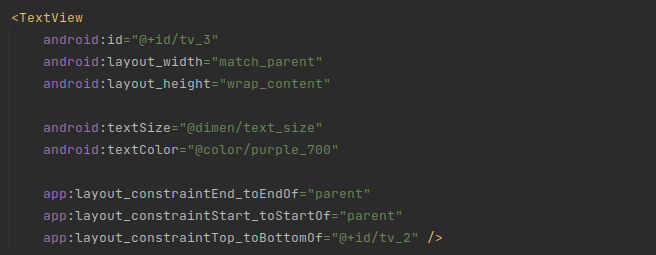
\includegraphics[width=0.9\textwidth]{Screenshot from 2023-03-30 19-31-39}
	\caption{Использование ресурсов colors в XML-коде}
	\label{fig:xml:color:use}
\end{image}

\begin{image}
	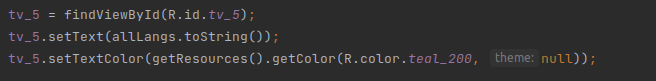
\includegraphics[width=0.9\textwidth]{Screenshot from 2023-03-30 19-40-51}
	\caption{Использование ресурсов colors в Java-коде}
	\label{fig:java:color:use}
\end{image}

\clearpage

\section*{\LARGE{Вывод}}
\addcontentsline{toc}{section}{Вывод}
В этой практической работе были получены знания для создания и
использования различный ресурсов. Освоены такие виды ресурсов как:

\begin{itemize}
	\item ресурсы строк;
	\item форматирование строк;
	\item ресурсы Plurals;
	\item ресурсы string array;
	\item ресурсы dimension;
	\item ресурсы Color.
\end{itemize}

